\section{Architectures: Fully Connected, Convolutional and Residual}\label{sec:arch}
In this section, we present the three architectures that we take up for theoretical analysis. These are i) fully connected (FC or FC-DNN), ii) convolutional (CNN) and iii) residual (ResNets). In what follows, $[n]$ is the set $\{1,\ldots,n\}$, and the dataset is given by $(x_s,y_s)_{s=1}^n\in\R^{\din}\times \R$.

\textbf{Fully Connected:} We consider fully connected networks with width `$w$' and depth `$d$'.
 \FloatBarrier
\begin{table}[h]
\centering
\begin{tabular}{|c l lll|}\hline
Input Layer&: &$z_{x,\Theta}(\cdot,0)$ &$=$ &$x$ \\
Pre-activation&: & $q_{x,\Theta}(\iout,l)$& $=$ & $\sum_{\iin}\Theta(\iin,\iout,l) \cdot z_{x,\Theta}(\iin,l-1) $\\
Gating Value&: &$G_{x,\Theta}(\iout,l)$& $=$ & $\mathbf{1}_{\{q_{x,\Theta}(\iout,l)>0\}}$\\
Hidden Unit Output&: &$z_{x,\Theta}(\iout,l)$ & $=$ & $q_{x,\Theta}(\iout,l)\cdot G_{x,\Theta}(\iout,l)$\\
Final Output&: & $\hat{y}_{\Theta}(x)$ & $=$ & $\sum_{\iin}\Theta(\iin,\iout, d)\cdot z_{x,\Theta}(\iin,d-1)$\\\hline
\end{tabular}
\caption{\small{Information flow in a FC-DNN with ReLU. Here, `$q$'s are pre-activation inputs, `$z$'s are output of the hidden layers, `$G$'s are the gating values. $l\in[d-1]$ is the index of the layer, $\iout$ and $\iin$ are indices of  nodes in the current and previous layer respectively.}}
\label{tb:basic}
\end{table}

\textbf{CNN:} We consider a $1$-dimensional convolutional neural network with circular convolutions (see \Cref{tb:cconv}), with $\dc$ convolutional layers ($l=1,\ldots,\dc$), followed by a \emph{global-average/max-pooling} layer ($l=\dc+1$) and $\dfc$ ($l=\dc+2,\ldots,\dc+\dfc+1$) FC  layers. The convolutional window size is $\wconv<\din$, the number of filters per convolutional layer is $w$, and the width of the FC is also $w$. 
\begin{definition}[Circular Convolution]
For $x\in\R^{\din}$, $i\in[\din]$ and $r\in\{0,\ldots,\din-1\}$, define :

(i) $i\oplus r = i+r$, for $i+r \leq \din$ and $i\oplus r =i+r-\din$, for $i+r>\din$.

(ii) $rot(x,r)(i)=x(i\oplus r), i\in[\din]$.

(iii) $q_{x,\Theta}(\ifout,\iout,l)=\sum_{\icin,\iin}\Theta(\icin,\iin,\iout,l)\cdot z_{x,\Theta}(\ifout\oplus (\icin-1),\iin,l-1)$, where $\iin/\iout$ are the indices (taking values in $[w]$) of the input/output filters. $\icin$ denotes the indices of the convolutional window (taking values in $[\wconv]$) between input and output filters $\iin$ and $\iout$. $\ifout$ denotes the indices (taking values in $[\din]$, the dimension of input features) of individual nodes in a given output filter.
\end{definition}
\begin{definition}[Pooling]
Let $G^{\text{pool}}_{x,\Theta}(\ifout,\iout,\dc+1)$ denote the pooling mask, then we have
\begin{align*}
z_{x,\Theta}(\iout, \dc+1) =\sum_{\ifout} z_{x,\Theta}(\ifout,\iout,\dc)\cdot G^{\text{pool}}_{x,\Theta}(\ifout,\iout,\dc+1),
\end{align*}
where in the case of \emph{global-average-pooling} $G^{\text{pool}}_{x,\Theta}(\ifout,\iout,\dc+1)=\frac{1}{\din},\forall \iout\in[w], \ifout\in[\din]$, and in the case of \emph{$\max$-pooling},  
for a given $\iout\in[w]$, $G^{\text{pool}}_{x,\Theta}(i_{\max},\iout,\dc+1)=1$ where $i_{\max}=\arg\max_{\ifout}z_{x,\Theta}(\ifout,\iout,\dc)$, and $G^{\text{pool}}_{x,\Theta}(\ifout,\iout,\dc+1)=0,\forall \ifout\neq i_{\max}$.
\end{definition}

\textbf{ResNet:} We consider ResNets with `$(b+2)$' blocks and `$b$' skip connections between the blocks (\Cref{fig:resnet}). Each block is a FC-DNN of depth `$\dblock$' and width `$w$'. Here, $\gamma^{\text{pre}}_i,\gamma^{\text{post}}_i,i\in[b]$ are normalisation variables. 
\begin{figure}
\centering
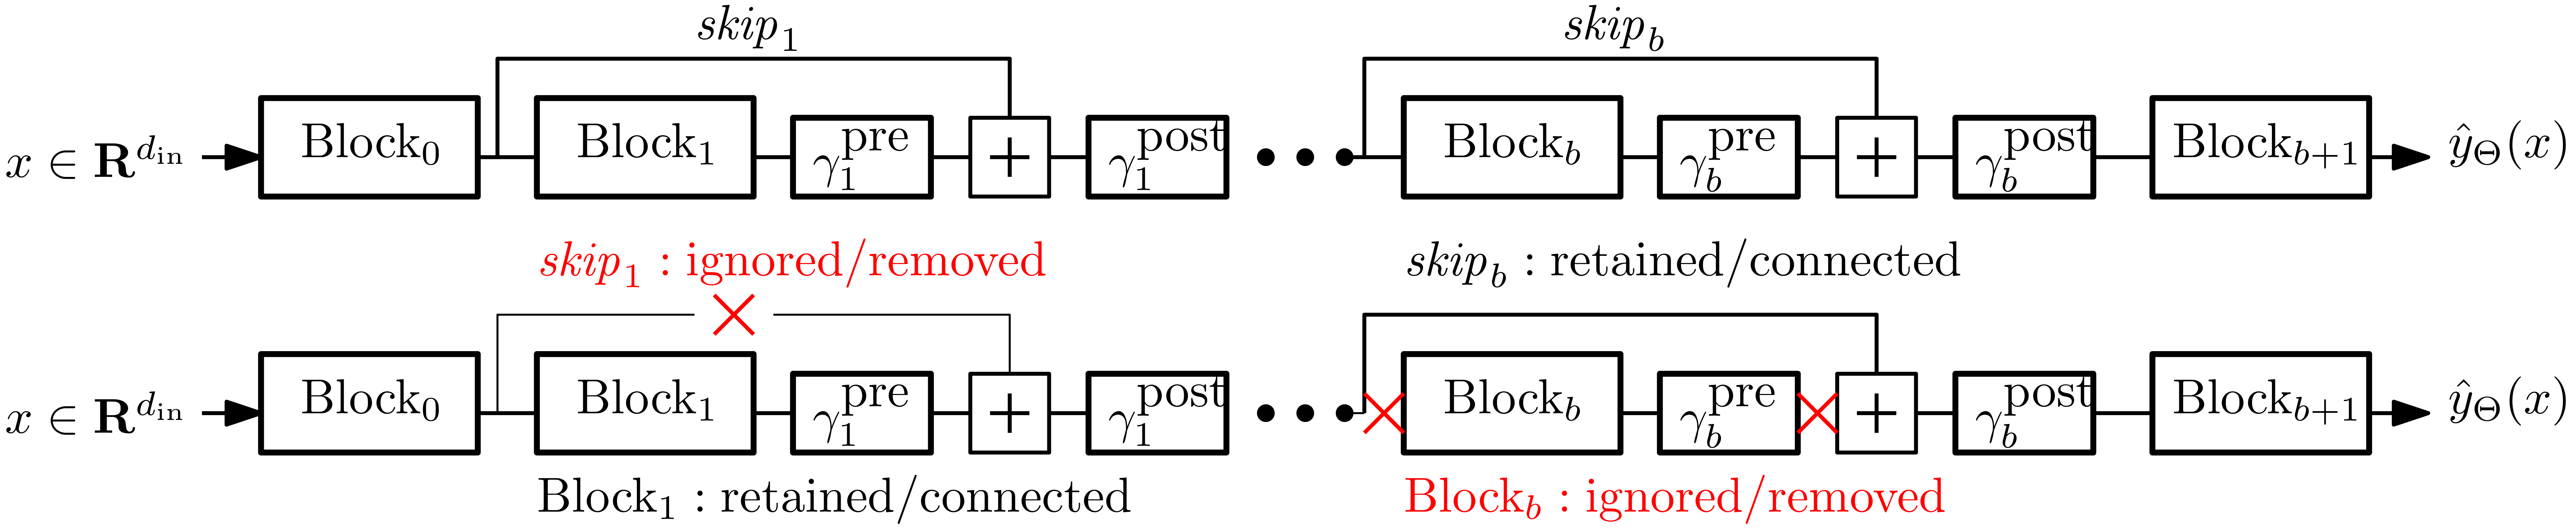
\includegraphics[scale=0.04]{figs/resnet-full.png}
\caption{\small{ResNet Architecture is shown in the top. Process of obtaining a sub-FC-DNN by ignoring skip (retaining block) or retaining skip (ignoring block) is shown in the bottom.}}
\label{fig:resnet}
\end{figure}
\begin{definition}[Sub FC-DNNs]
Let $2^{[b]}$ denote the power set of $[b]$ and let $\J\in 2^{[b]}$ denote any subset of $[b]$. Define the`$\J^{th}$' sub-FC-DNN of the ResNet to be the fully connected network obtained by ignoring/removing (see \Cref{fig:resnet}) the skip connections $\text{skip}_j,\forall j\in \J$ (see \Cref{fig:resnet}).
\end{definition}
\begin{comment}
\FloatBarrier
\begin{figure}[h]
\resizebox{\columnwidth}{!}{
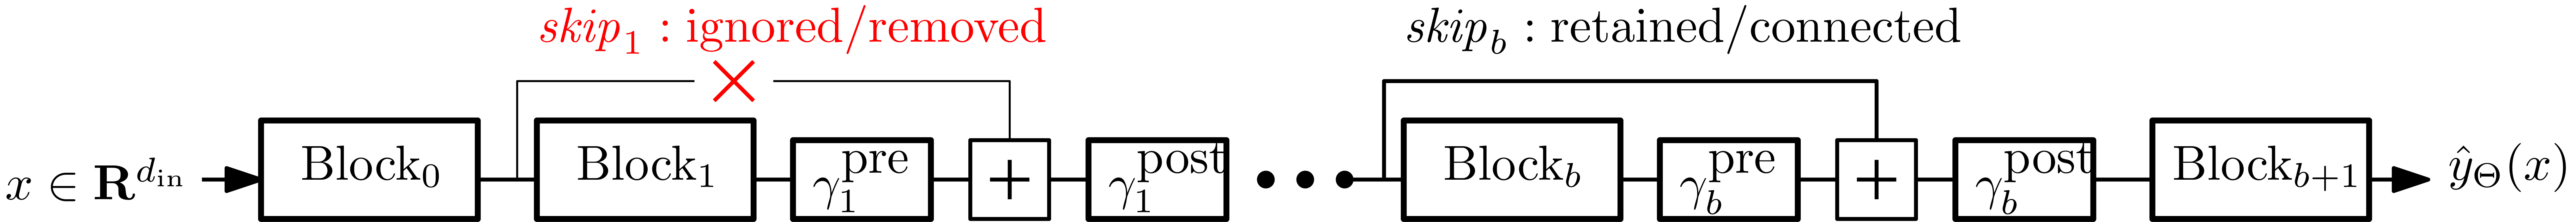
\includegraphics{figs/resnet-ignore.png}
}
\caption{Sub-FC-DNNs within a ResNet.}
\label{fig:resnet-ignore}
\end{figure}
\end{comment}

